%!TEX root = ../thesis.tex

%%%%%%%%%%%%%%%%%%%%%%%%
%    STANDARD MODEL    %
%%%%%%%%%%%%%%%%%%%%%%%%

\message{^^J ^^J STANDARD MODEL ^^J ^^J} % print to log
\newchap{The Standard Model}\label{sec:SM}

This chapter introduces the Standard Model (SM) of particle physics.
I left a bit of text with equations, citations, figures, and tables as an example of this template.


%%%%%%%%%%%%%%%%%%%%%%%%
%    STANDARD MODEL    %
%%%%%%%%%%%%%%%%%%%%%%%%
\section{The Standard Model}

A rough timeline of the experimental discovery of particles is given by \Fig{fig:timeline}.
More detailed historical discussions can be found in Refs.~\cite{particle_physics_history_50s,particle_physics_history_60s,particle_physics_Griffiths}.

% FIG: timeline
%!TEX root = ../thesis.tex

% FIGURE: hierarchy problem - SM
\begin{figure*}[p]
  %\vspace{-3mm}
  \centerline{
    \includegraphics[width=1.0\textwidth,page=2]{fig/intro/SM_timeline.pdf}
  }
  \caption{
A timeline of particle physics in the last 130 years.
Adapted from Ref.~\cite{particle_physics_timeline_fig}.
  } \label{fig:timeline}
  %\vspace*{-2mm}
\end{figure*}


With a mass of $m_\PQt\approx172.8\GeV$~\cite[p.~32]{PDG_2022}, the top quark is by far the heaviest fermion.

The discovery of the Higgs was announced in 2012~\cite{Higgs_discovery_2012_CMS,Higgs_discovery_2012_ATLAS,Higgs_discovery_2013_CMS,Higgs_mass_2015_combined}. A single Higgs boson is the simplest and most minimal solution, although it is possible to achieve SBB with more than one Higgs boson. No evidence of additional Higgs bosons have been found so far~\cite{Higgs_extensions_LHC_2021}.

% FIG: SM overview
%!TEX root = ../thesis.tex

% FIGURE: SM particle content
\begin{figure*}[p]
  %\vspace{-12mm}
  \centering
  %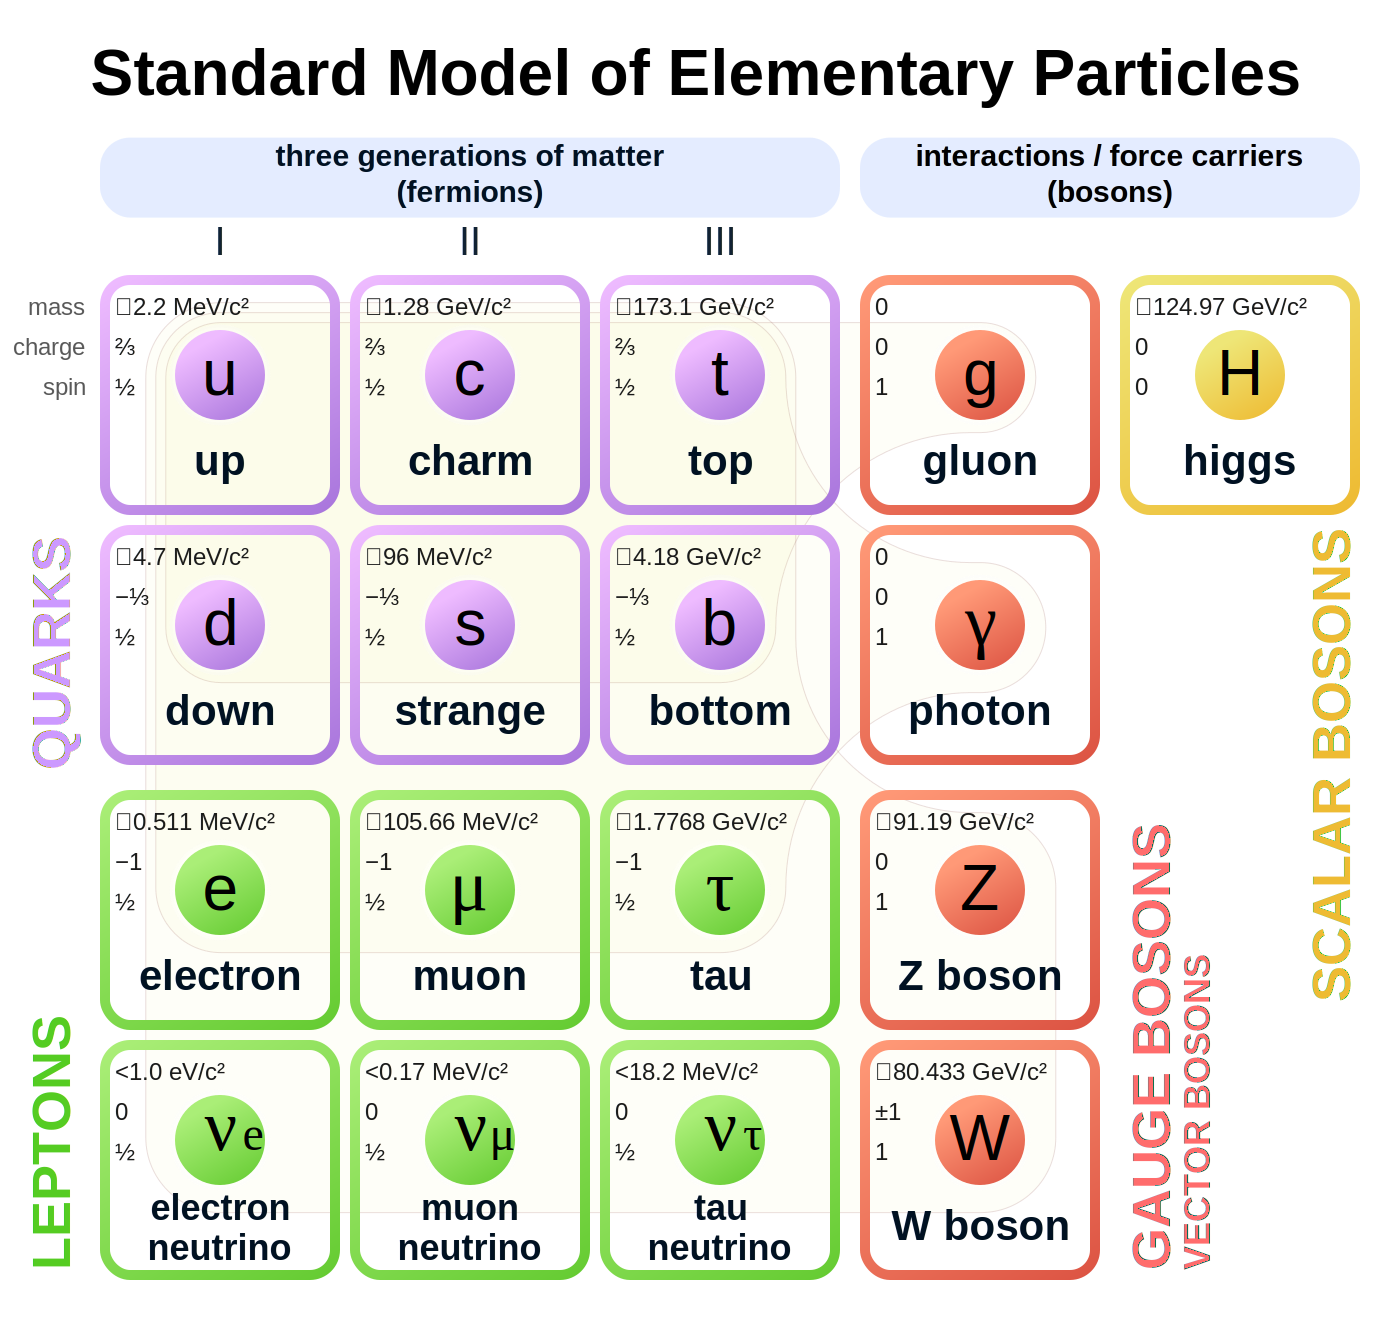
\includegraphics[width=0.6\textwidth,clip,trim={0mm 0mm 0mm 40mm}]{fig/intro/SM_particles_Wiki.pdf}
  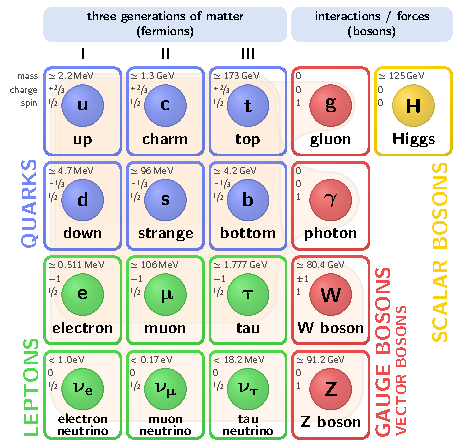
\includegraphics[width=0.6\textwidth]{fig/intro/SM_particles.pdf}
  %\vspace{-1mm}
  \caption{
A table of the particles in Standard Model of particle physics and their properties.
Figure adapted from Ref.~\cite{SM_fig}.
  } \label{fig:SM_particles}
  \vspace*{-6mm}
\end{figure*}


% LAGRANGIAN
\subsection{The Standard Model Lagrangian}
The SM is encoded in the \emph{SM Lagrangian density}.
The terms of the Lagrangian density can be grouped into three separate \emph{sectors}:
\begin{equation}
  \Lg{SM} = \Lg{gauge} + \Lg{Higgs} + \Lg{Yukawa}.
\end{equation}

Secondly, the SM is a \emph{gauge theory}: It has an internal symmetry that corresponds to the local $\GSM$ symmetry group.
The SM gauge group is spontaneously broken to
\begin{equation}
  \GSM \;\xrightarrow{\mathrm{SSB}}\; \SU[C]{3}\times\U[EM]{1}
\end{equation}
by the nonzero vev of the Higgs field, where $\U[EM]{1}$ is the gauge symmetry group for QED.

% GAUGE SECTOR
\subsection{The gauge sector} \label{sec:gauge}
The gauge sector can be written as
\begin{align} \label{eq:gauge}
  \Lg{gauge} &= \sum_f \sum_{\psi_f} \overline{\psi}_f i\gamma^\mu D_\mu \psi_f %\\ %\slashed{D}
              -\frac{1}{4} G^a_{\mu\nu}G_a^{\mu\nu}
              -\frac{1}{4} W^i_{\mu\nu}W_i^{\mu\nu}
              -\frac{1}{4} B^{\mu\nu}B^{\mu\nu},
\end{align}
in natural units $c=\hbar=1$~\cite{flavor_lecture_Isidori_UZH}, and where $a=1,...,8$ and $i=1,2,3$.
In the first term, matter is given by five fermion fields $\psi_f$ in three generations $f=1,2,3$;
\begin{equation} \label{eq:matter}
  \ff{Q}{L}^f = \db{\ff{u^f}{L}}{\ff{d^f}{L}},\quad
  \ff{u}{R}^f,\quad
  \ff{d}{R}^f,\quad
  \ff{L}{L}^f = \db{\ff{\nu^f}{L}}{\ff{e^f}{L}},\quad
  \ff{e}{R}^f.
\end{equation}
Their Dirac adjoints are given by $\overline{\psi}_f = \psi_f^\dagger\gamma^0$.

% FIGURE: SM fields
%!TEX root = ../thesis.tex

% TABLE: SM Summary
%   https://en.wikipedia.org/wiki/File:Electroweak.svg
%   https://commons.wikimedia.org/wiki/File:Standard_Model.svg
%   https://en.wikipedia.org/wiki/Mathematical_formulation_of_the_Standard_Model#Field_content_in_detail
\begin{table}[p]
\vspace*{-6mm}
\centering
\caption{
Summary of the representation and quantum numbers SM fields.
Bold numbers indicate the dimension of the representation under the respective gauge group.
}\label{tab:SM_symmetries}
\def\arraystretch{1.3}
\def\vsdb{\rule[-15pt]{0pt}{36pt}} % vertical space for doublet
\begin{tabular}{llc@{\extracolsep{\tabcolsep}}c@{\extracolsep{4pt}}c@{\extracolsep{\tabcolsep}}c@{\extracolsep{1.5\tabcolsep}}c}
  \hline
  %Field name  & Symbol      & $\SU[C]{3}$ & $\SU[L]{2}$ & $T_3$ & $\YW/2$ & $Q = T_3 + \YW/2$ \\
  \multirow{2}{*}{Field name}
        & \multirow{2}{*}{Symbol}
               & \multicolumn{2}{c}{Representations} & \multicolumn{3}{c}{Quantum numbers} \\
                 \cline{3-4}                           \cline{5-7}
        &      & $\SU[C]{3}$ & $\SU[L]{2}$ & $T_3$ & $\YW/2$ & $Q = T_3 + \YW/2$ \\
  \hline
  \vsdb % add vertical space above & below
  Quark doublet
        & $\ff{Q}{L} = \db{\ff{u}{L}}{[1pt]\ff{d}{L}}$
               & \textbf{3}  & \textbf{2} & $\db{+\frac{1}{2}}{[2pt]-\frac{1}{2}}$
                                                   & $+\frac{1}{6}$
                                                             & $\db{+\frac{2}{3}}{[2pt]-\frac{1}{3}}$ \\[2mm]
  Up-quark singlet
        & $\ff{u}{R}$  & \textbf{3}  & \textbf{1} & $+\frac{2}{3}$
                                                   & $+\frac{2}{3}$
                                                             & $+\frac{2}{3}$ \\
  Down-quark singlet
        & $\ff{d}{R}$  & \textbf{3}  & \textbf{1} & $-\frac{1}{3}$
                                                   & $-\frac{1}{3}$
                                                             & $-\frac{2}{3}$ \\
  \vsdb % add vertical space above & below
  Lepton doublet
        & $\ff{L}{L} = \db{\ff{\nu}{L}}{[1pt]\ff{e}{L}}$ 
                       & \textbf{1}  & \textbf{2} & $\db{+\frac{1}{2}}{[2pt]-\frac{1}{2}}$
                                                   & $-\frac{1}{2}$
                                                             & $\db{\phmin0}{-1}$ \\[2mm]
  Lepton singlet
        & $\ff{e}{R}$  & \textbf{1}  & \textbf{1} & $\phmin0$
                                                   & $-1$    & $-1$ \\
  \hline
  Gluon field
        & $G^a_\mu$    & \textbf{8}  & \textbf{1} & $\phmin0$
                                                   & $\phmin0$ & $\phmin0$ \\
  \rule[-19pt]{0pt}{42pt}% % add vertical space above & below
  Weak gauge field
        & $W^i_\mu = \db{W^+_\mu}{W^-_\mu\\W^3_\mu}$
                       & \textbf{1}  & \textbf{3} & $\db{+1}{-1\\\phmin0}$
                                                   & $\phmin0$ & $\db{+1}{-1\\\phmin0}$\\
  Hypercharge field
        & $B_\mu$
                       & \textbf{1}  & \textbf{1} & $\phmin0$
                                                   & $\phmin0$ & $\phmin0$ \\
%  Weak gauge bosons
%        & $\db{W^+_\mu}{W^-_\mu\\Z^0_\mu}$
%               & \textbf{1}  & \textbf{3} & $\db{+1}{-1\\0}$
%                                                   & \phmin0 & $\db{+1}{-1\\\phmin0}$\\
%  Photon
%        & $A^a_\mu$    & \textbf{1}  & \textbf{1} & $\phmin0$
%                                                   & $\phmin0$ & $\phmin0$ \\
  \hline
  \vsdb % add vertical space above & below
  Higgs doublet
        & $\Phi = \db{\phi^+}{[1pt]\phi^0}$
               & \textbf{1}  & \textbf{2} & $\db{+\frac{1}{2}}{[2pt]-\frac{1}{2}}$
                                                   & $+\frac{1}{2}$
                                                             & $\db{+1}{\phmin0}$ \\[2mm]
  \vsdb % add vertical space above & below
  Conjugate Higgs doublet
        & $\Phi^\mathrm{c} = \db{\phi^{0*}}{[1pt]\phi^-}$
               & \textbf{1}  & \textbf{2} & $\db{+\frac{1}{2}}{[2pt]-\frac{1}{2}}$
                                                   & $-\frac{1}{2}$
                                                             & $\db{\phmin0}{-1}$ \\[2mm]
  \hline
\end{tabular}
\end{table}

%!TEX root = ../thesis.tex

% TABLE: SM Summary
%   https://en.wikipedia.org/wiki/File:Electroweak.svg
%   https://commons.wikimedia.org/wiki/File:Standard_Model.svg
%   https://en.wikipedia.org/wiki/Mathematical_formulation_of_the_Standard_Model#Field_content_in_detail
\begin{table}[p]
\vspace*{-6mm}
\centering
\caption{
Summary of the representation and quantum numbers SM fields.
Bold numbers indicate the dimension of the representation under the respective gauge group.
}\label{tab:SM_symmetries}
\def\arraystretch{1.3}
\def\vsdb{\rule[-15pt]{0pt}{36pt}} % vertical space for doublet
\begin{tabular}{llc@{\extracolsep{\tabcolsep}}c@{\extracolsep{4pt}}c@{\extracolsep{\tabcolsep}}c@{\extracolsep{1.5\tabcolsep}}c}
  \hline
  %Field name  & Symbol      & $\SU[C]{3}$ & $\SU[L]{2}$ & $T_3$ & $\YW/2$ & $Q = T_3 + \YW/2$ \\
  \multirow{2}{*}{Field name}
        & \multirow{2}{*}{Symbol}
               & \multicolumn{2}{c}{Representations} & \multicolumn{3}{c}{Quantum numbers} \\
                 \cline{3-4}                           \cline{5-7}
        &      & $\SU[C]{3}$ & $\SU[L]{2}$ & $T_3$ & $\YW/2$ & $Q = T_3 + \YW/2$ \\
  \hline
  \vsdb % add vertical space above & below
  Quark doublet
        & $\ff{Q}{L} = \db{\ff{u}{L}}{[1pt]\ff{d}{L}}$
               & \textbf{3}  & \textbf{2} & $\db{+\frac{1}{2}}{[2pt]-\frac{1}{2}}$
                                                   & $+\frac{1}{6}$
                                                             & $\db{+\frac{2}{3}}{[2pt]-\frac{1}{3}}$ \\[2mm]
  Up-quark singlet
        & $\ff{u}{R}$  & \textbf{3}  & \textbf{1} & $+\frac{2}{3}$
                                                   & $+\frac{2}{3}$
                                                             & $+\frac{2}{3}$ \\
  Down-quark singlet
        & $\ff{d}{R}$  & \textbf{3}  & \textbf{1} & $-\frac{1}{3}$
                                                   & $-\frac{1}{3}$
                                                             & $-\frac{2}{3}$ \\
  \vsdb % add vertical space above & below
  Lepton doublet
        & $\ff{L}{L} = \db{\ff{\nu}{L}}{[1pt]\ff{e}{L}}$ 
                       & \textbf{1}  & \textbf{2} & $\db{+\frac{1}{2}}{[2pt]-\frac{1}{2}}$
                                                   & $-\frac{1}{2}$
                                                             & $\db{\phmin0}{-1}$ \\[2mm]
  Lepton singlet
        & $\ff{e}{R}$  & \textbf{1}  & \textbf{1} & $\phmin0$
                                                   & $-1$    & $-1$ \\
  \hline
  Gluon field
        & $G^a_\mu$    & \textbf{8}  & \textbf{1} & $\phmin0$
                                                   & $\phmin0$ & $\phmin0$ \\
  \rule[-19pt]{0pt}{42pt}% % add vertical space above & below
  Weak gauge field
        & $W^i_\mu = \db{W^+_\mu}{W^-_\mu\\W^3_\mu}$
                       & \textbf{1}  & \textbf{3} & $\db{+1}{-1\\\phmin0}$
                                                   & $\phmin0$ & $\db{+1}{-1\\\phmin0}$\\
  Hypercharge field
        & $B_\mu$
                       & \textbf{1}  & \textbf{1} & $\phmin0$
                                                   & $\phmin0$ & $\phmin0$ \\
%  Weak gauge bosons
%        & $\db{W^+_\mu}{W^-_\mu\\Z^0_\mu}$
%               & \textbf{1}  & \textbf{3} & $\db{+1}{-1\\0}$
%                                                   & \phmin0 & $\db{+1}{-1\\\phmin0}$\\
%  Photon
%        & $A^a_\mu$    & \textbf{1}  & \textbf{1} & $\phmin0$
%                                                   & $\phmin0$ & $\phmin0$ \\
  \hline
  \vsdb % add vertical space above & below
  Higgs doublet
        & $\Phi = \db{\phi^+}{[1pt]\phi^0}$
               & \textbf{1}  & \textbf{2} & $\db{+\frac{1}{2}}{[2pt]-\frac{1}{2}}$
                                                   & $+\frac{1}{2}$
                                                             & $\db{+1}{\phmin0}$ \\[2mm]
  \vsdb % add vertical space above & below
  Conjugate Higgs doublet
        & $\Phi^\mathrm{c} = \db{\phi^{0*}}{[1pt]\phi^-}$
               & \textbf{1}  & \textbf{2} & $\db{+\frac{1}{2}}{[2pt]-\frac{1}{2}}$
                                                   & $-\frac{1}{2}$
                                                             & $\db{\phmin0}{-1}$ \\[2mm]
  \hline
\end{tabular}
\end{table}


% FIG: SM Summary
\begin{figure*}[p]
  \vspace*{-10mm}
  \centerline{
    \includegraphics[height=0.56\linewidth,page=5]{fig/intro/SM_isospin_weak.pdf}
    \includegraphics[height=0.56\linewidth,page=4]{fig/intro/SM_isospin_weak.pdf}
  }
  \caption{
Graph of the $(T_3,\YW/2)$ quantum numbers.
  }\label{fig:SM_quantum_numbers_fermions}
  \vspace*{-6mm}
\end{figure*}


The covariant derivative
\begin{equation}
  D_\mu = \partial_\mu
          + ig_\mathrm{s}t_aG^a_\mu
          + igT_iW^i_\mu
          + ig'\frac{Y}{2}B_\mu
\end{equation}
where $T_i$ and $t_a$ and are the generators for $\SU[L]{2}$ and $\SU[C]{3}$, respectively, and $Y$ is the weak hypercharge of the field that $D_\mu$ acts on.

Through the Higgs mechanism, the gauge bosons acquire mass and mix into the mass eigenstates
\begin{equation}
  W^\pm_\mu = \frac{W^1_\mu \mp iW^2_\mu}{\sqrt{2}},\quad
  Z_\mu = W^3_\mu\cos\thetaW + B^3_\mu\sin\thetaW,\quad
  A_\mu = W^3_\mu\sin\thetaW - B^3_\mu\cos\thetaW,
\end{equation}
where $W^\pm_\mu$ are the charged W boson fields,
$Z_\mu$ is the neutral Z boson field,
$A_\mu$ is the photon field,
and $\thetaW$ is the Weinberg angle given by $\sin\thetaW = g'/\sqrt{g^2+g'^2}$.
After mixing, the new covariant derivative becomes
\begin{equation} \label{eq:D_mu_broken}
  D_\mu = \partial_\mu
          + ig_\mathrm{s}t_aG^a_\mu
          + i\frac{g}{\sqrt{2}}T^+W^+_\mu
          + i\frac{g}{\sqrt{2}}T^-W^-_\mu
          + i\frac{g}{\cos\thetaW}\left( T_3 - \sin^2{\thetaW}\, Q \right)Z_\mu
          + ieQA_\mu,
\end{equation}
with ladder operators $T^\pm = T_1 \pm iT_2$.


% YUKAWA SECTOR
\subsection{The Yukawa sector} \label{sec:Yukawa}
In order to explain mass of the fermions,
\begin{equation} \label{eq:Yukawa}
  \Lg{Yukawa}
  = -Y_d^{fg} \aff{Q}{L}^f\Phi\ff{d^g}{R}
    -Y_u^{fg} \aff{Q}{L}^f\Phi^\mathrm{c}\ff{u^g}{R}
    -Y_e^{fg} \aff{L}{L}^f\Phi\ff{e^g}{R}
    + \hc,
\end{equation}
with the conjugate Higgs doublet $\Phi^\mathrm{c}=i\sigma_2\Phi^\dagger$,
and unitary Yukawa matrices $Y_d^{fg}$, $Y_u^{fg}$, $Y_e^{fg} \in \U{3}$ that mixes the fermion generations.
As $\Phi$ is a scalar field that forms a weak isospin doublet,
\begin{equation}
  \Phi = \db{\phi^+}{\phi^0}.
\end{equation}

Because the Higgs vev is nonzero, we can fix the $\SU[L]{2}$ gauge.
It is convenient to choose the unitary gauge
\begin{equation}
  \Phi = \frac{1}{\sqrt{2}} \db{0}{v+h},
\end{equation}
with the vev $v\approx246\GeV$, a real constant, and the neutral Higgs field $h$, a (real) scalar.
Therefore, after SSB, we are left with
\begin{equation} \label{eq:Yukawa-mass}
  \Lg{Yukawa}
  = -\frac{Y_d^{fg}}{\sqrt{2}} \aff{d}{L}^f(v+h)\ff{d^g}{R}
    -\frac{Y_u^{fg}}{\sqrt{2}} \aff{u}{L}^f(v+h)\ff{u^g}{R}
    -\frac{Y_e^{fg}}{\sqrt{2}} \aff{e}{L}^f(v+h)\ff{e^g}{R}
    + \hc
\end{equation}


% CKM matrix
\subsection{CKM matrix}

% Cabibbo angle
To explain the suppressed decay rate of $\PK^0\to\PGm^+\PGm^-$, Glashow, Iliopoulos, and Maiani used a mixing matrix and proposed the existence of the charm quark~\cite{GIM}.
This is referred to as the \emph{Glashow–Iliopoulos–Maiani} (GIM) \emph{mechanism}.
The mixing of two quark generations is given by the \emph{Cabibbo matrix}:
\begin{equation} \label{eq:Cabibbo_matrix}
  \db{d'}{s'} = \begin{pmatrix}\phantom{-}
     \cos\thetaC & \sin\thetaC \\
    -\sin\thetaC & \cos\thetaC
  \end{pmatrix} \db{d}{s},
\end{equation}
where $\ket{d'}$ and $\ket{s'}$ represent the weak eigenstates, which are linear combinations of the mass eigenstates $\ket{d}$ and $\ket{s}$.
The mixing is quantified with the \emph{Cabibbo angle} $\thetaC\approx13.04^\circ$.

% CP-violation (neutral kaon system)
The mixing of three generations is given by
\begin{equation} \label{eq:CKM_matrix}
  \begin{pmatrix}
     d' \\
     s' \\
     b'
  \end{pmatrix} = \begin{pmatrix}
     V_{ud} & V_{us} & V_{ub} \\
     V_{cd} & V_{cs} & V_{cb} \\
     V_{td} & V_{ts} & V_{tb}
  \end{pmatrix} \begin{pmatrix}
     d \\
     s \\
     b
  \end{pmatrix},
\end{equation}
where the matrix is the so-called \emph{Cabbibo-Kobayashi-Maskawa} (CKM) \emph{matrix}, denoted by $\VCKM$.


% PROTON-PROTON COLLISIONS
\section{Higgs} \label{sec:Higgs}

A pie chart of Higgs decay can be found in \Fig{fig:Higgs_decay_piechart}.

% FIGURE: Higgs decay
%!TEX root = ../thesis.tex

% FIGURE: Higgs decay pie chart
\begin{figure*}[tbp]
  %\vspace{-6mm}
  \centering
  \includegraphics[width=0.41\textwidth,page=10]{fig/objects/SM_decay_piechart.pdf}
  \vspace{-1mm}
  \caption{
Pie chart of Higgs branching fractions.
Adapted from Ref.~\cite{branching_fractions_fig}.
%Numbers from PDG~\cite[p.~28]{PDG_2022}.
  } \label{fig:Higgs_decay_piechart}
  %\vspace{-3mm}
\end{figure*}



%%%%%%%%%%%%%%%%%%%%%%%%%%%%%%
%  PROTON-PROTON COLLISIONS  %
%%%%%%%%%%%%%%%%%%%%%%%%%%%%%%

% PROTON-PROTON COLLISIONS
\section{The physics of proton-proton collisions} \label{sec:pp_collisions}

The substructure of the proton has been carefully studied in deep inelastic scattering (DIS) experiments at SLAC~\cite{DIS_SLAC1,DIS_SLAC2} and DESY~\cite{DIS_HERA}, which collided electrons or positrons with protons.

In the parton model, \emph{parton distribution functions} (PDFs) describe the probability of finding a parton of type $p$ with momentum fraction $x$ in a collision at some momentum scale $Q$ as a function of the form $f_p(x,Q^2)$~\cite{parton_model1,parton_model2,parton_model_pp,pdfs,LHC_pdfs}.
The proton has \emph{valence quarks} and \emph{sea quarks}.
To reflect the proton quantum numbers, the PDFs are normalized:
\begin{equation}
  \int_0^1 \left[ f_\PQu(x,Q^2) - f_\PAQu(x,Q^2) \right] \dd{x} = 2, \quad
  \int_0^1 \left[ f_\PQd(x,Q^2) - f_\PAQd(x,Q^2) \right] \dd{x} = 1.
\end{equation}

% FIGURE: PDFs
%!TEX root = ../thesis.tex

% FIGURE: pp: pdfs
\begin{figure*}[t!]
  %\vspace{-3mm}
  \centering
  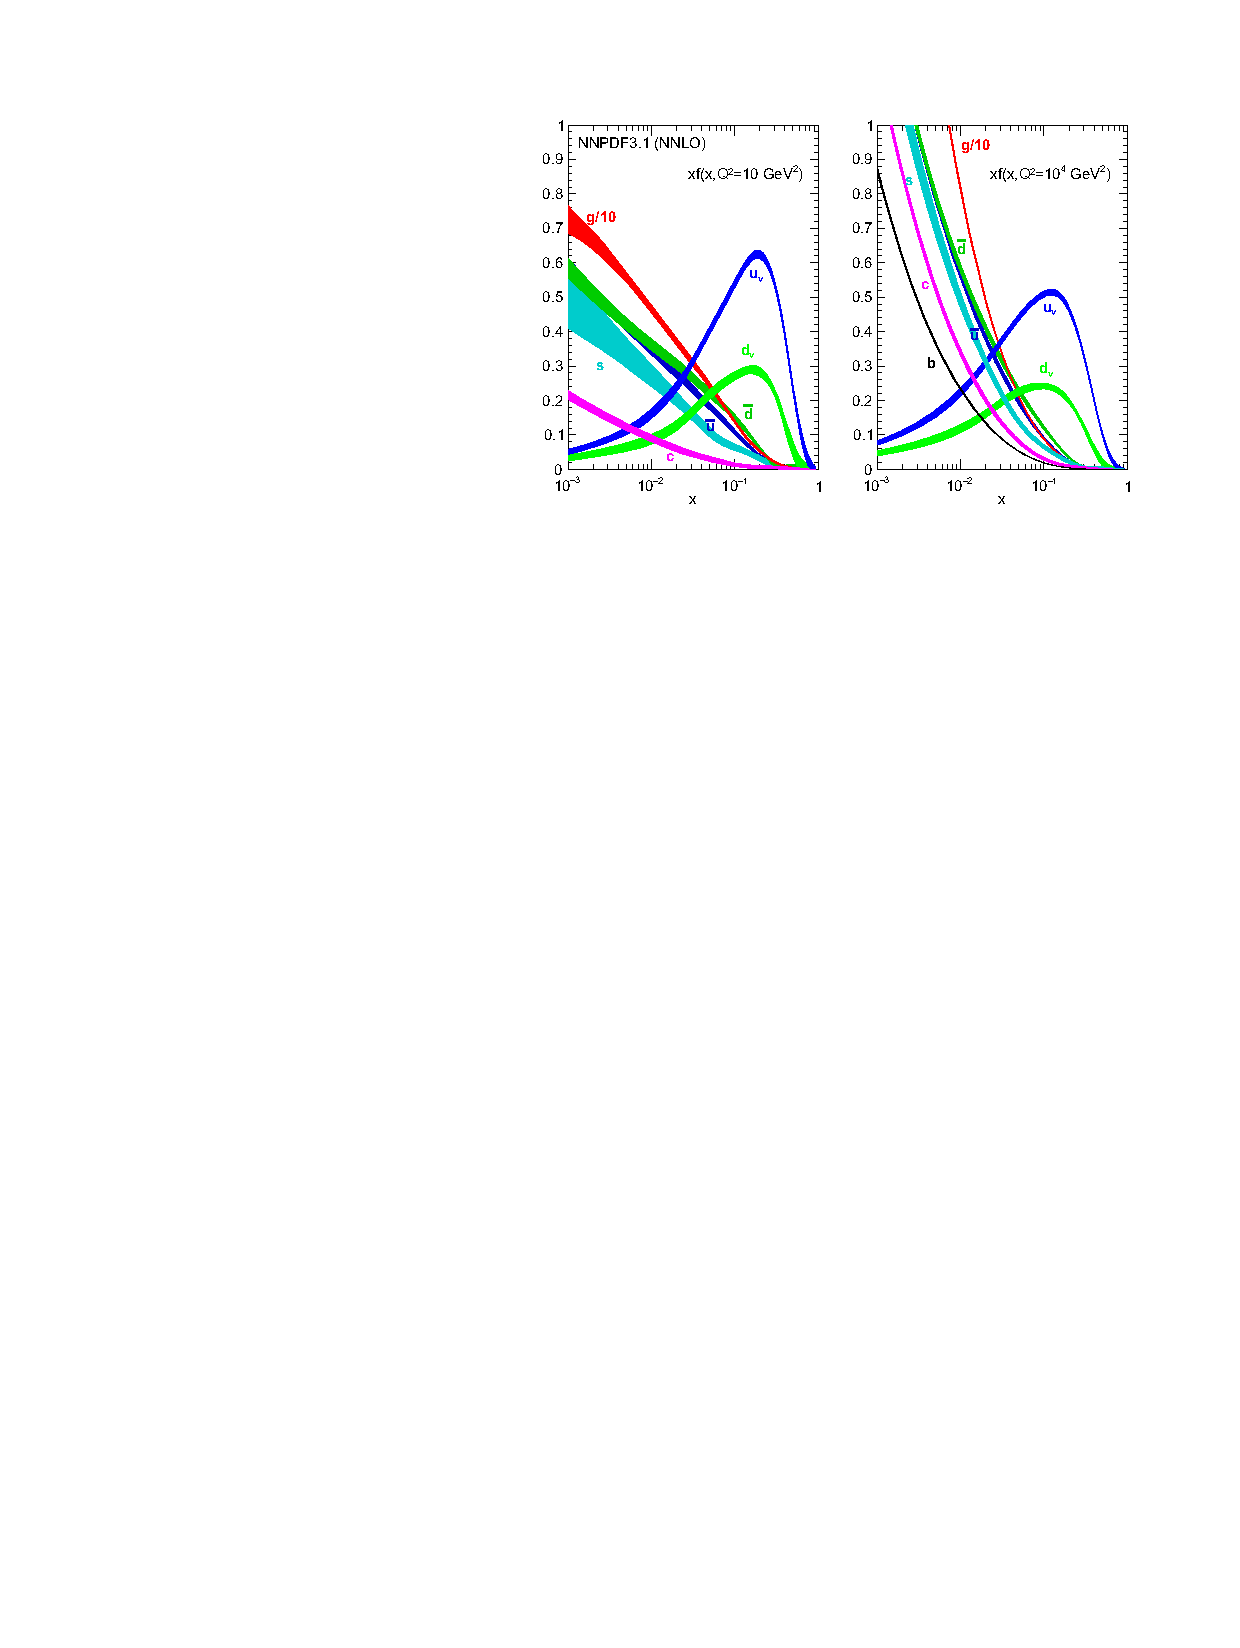
\includegraphics[height=8cm]{fig/intro/pdf_NNPDF3.1_NNLO.pdf}
  %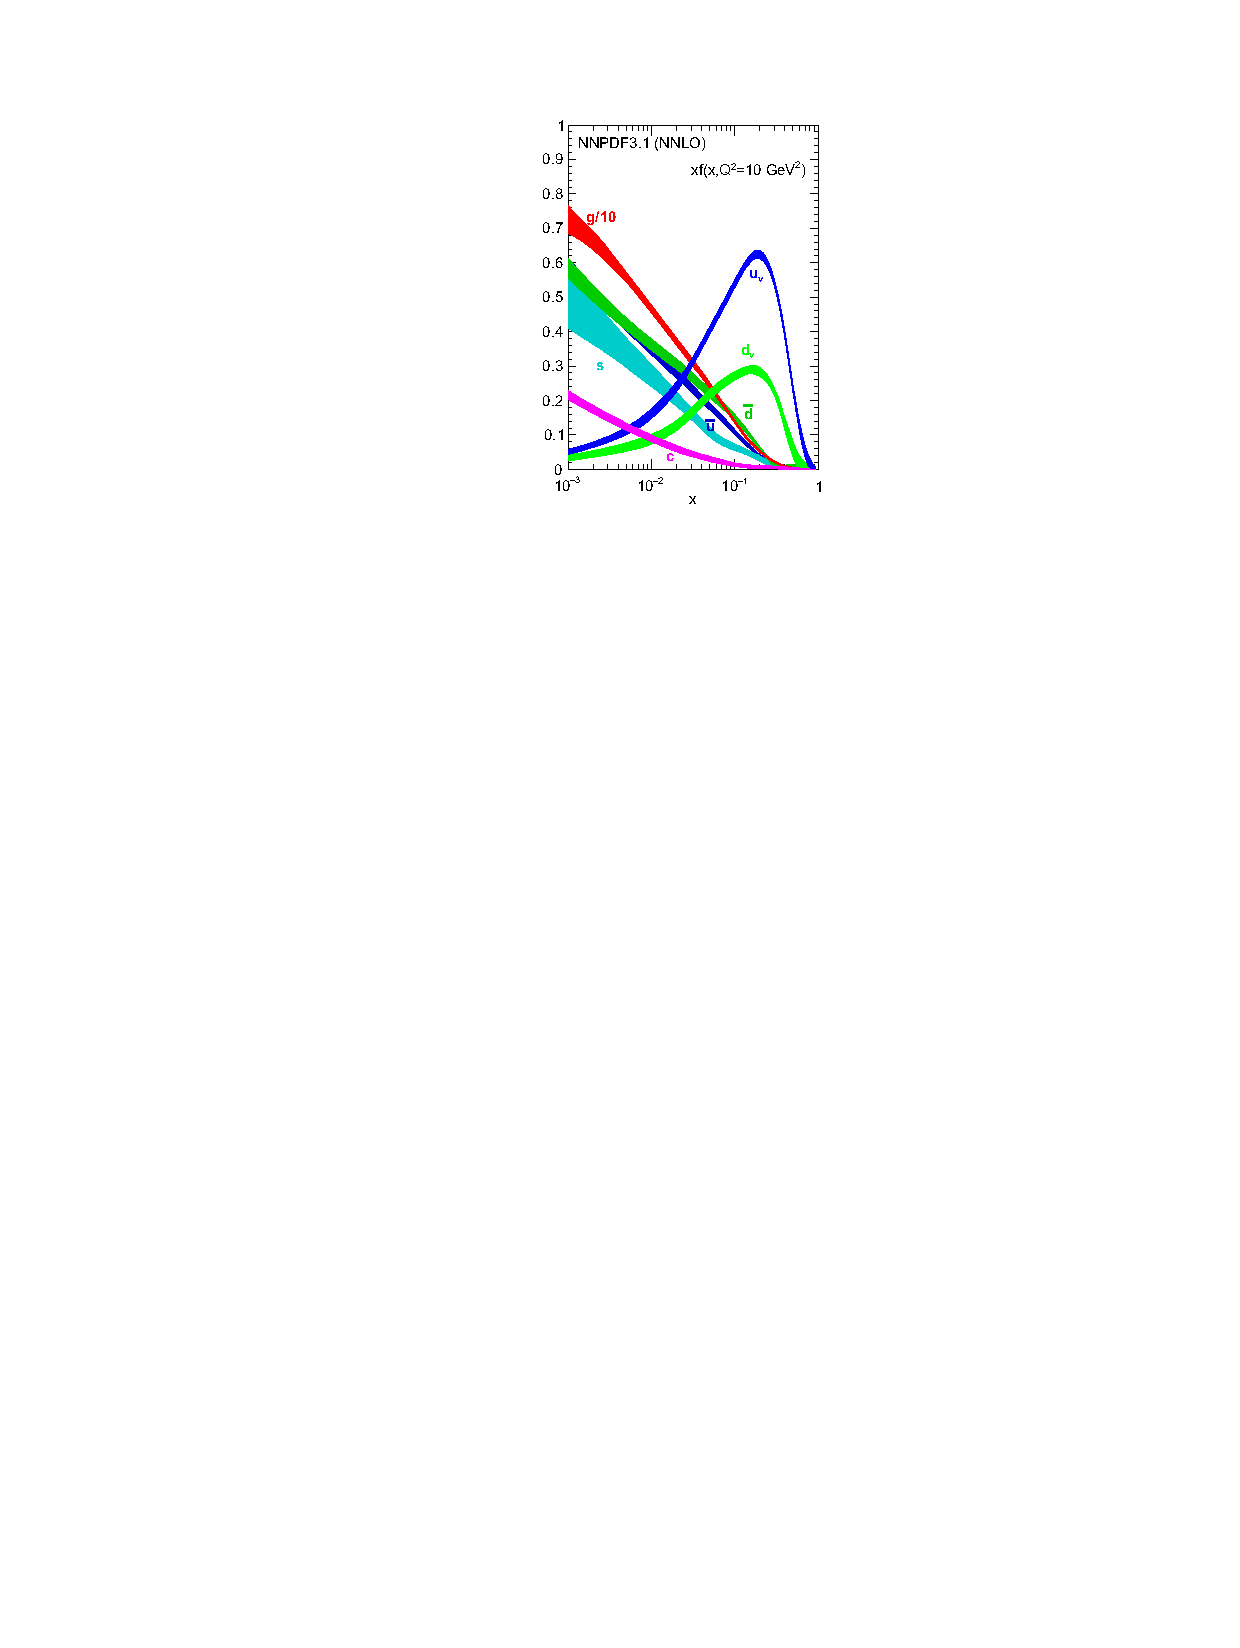
\includegraphics[height=7.8cm]{fig/intro/pdf_NNPDF3.1_NNLO_Q2-10.pdf}
  %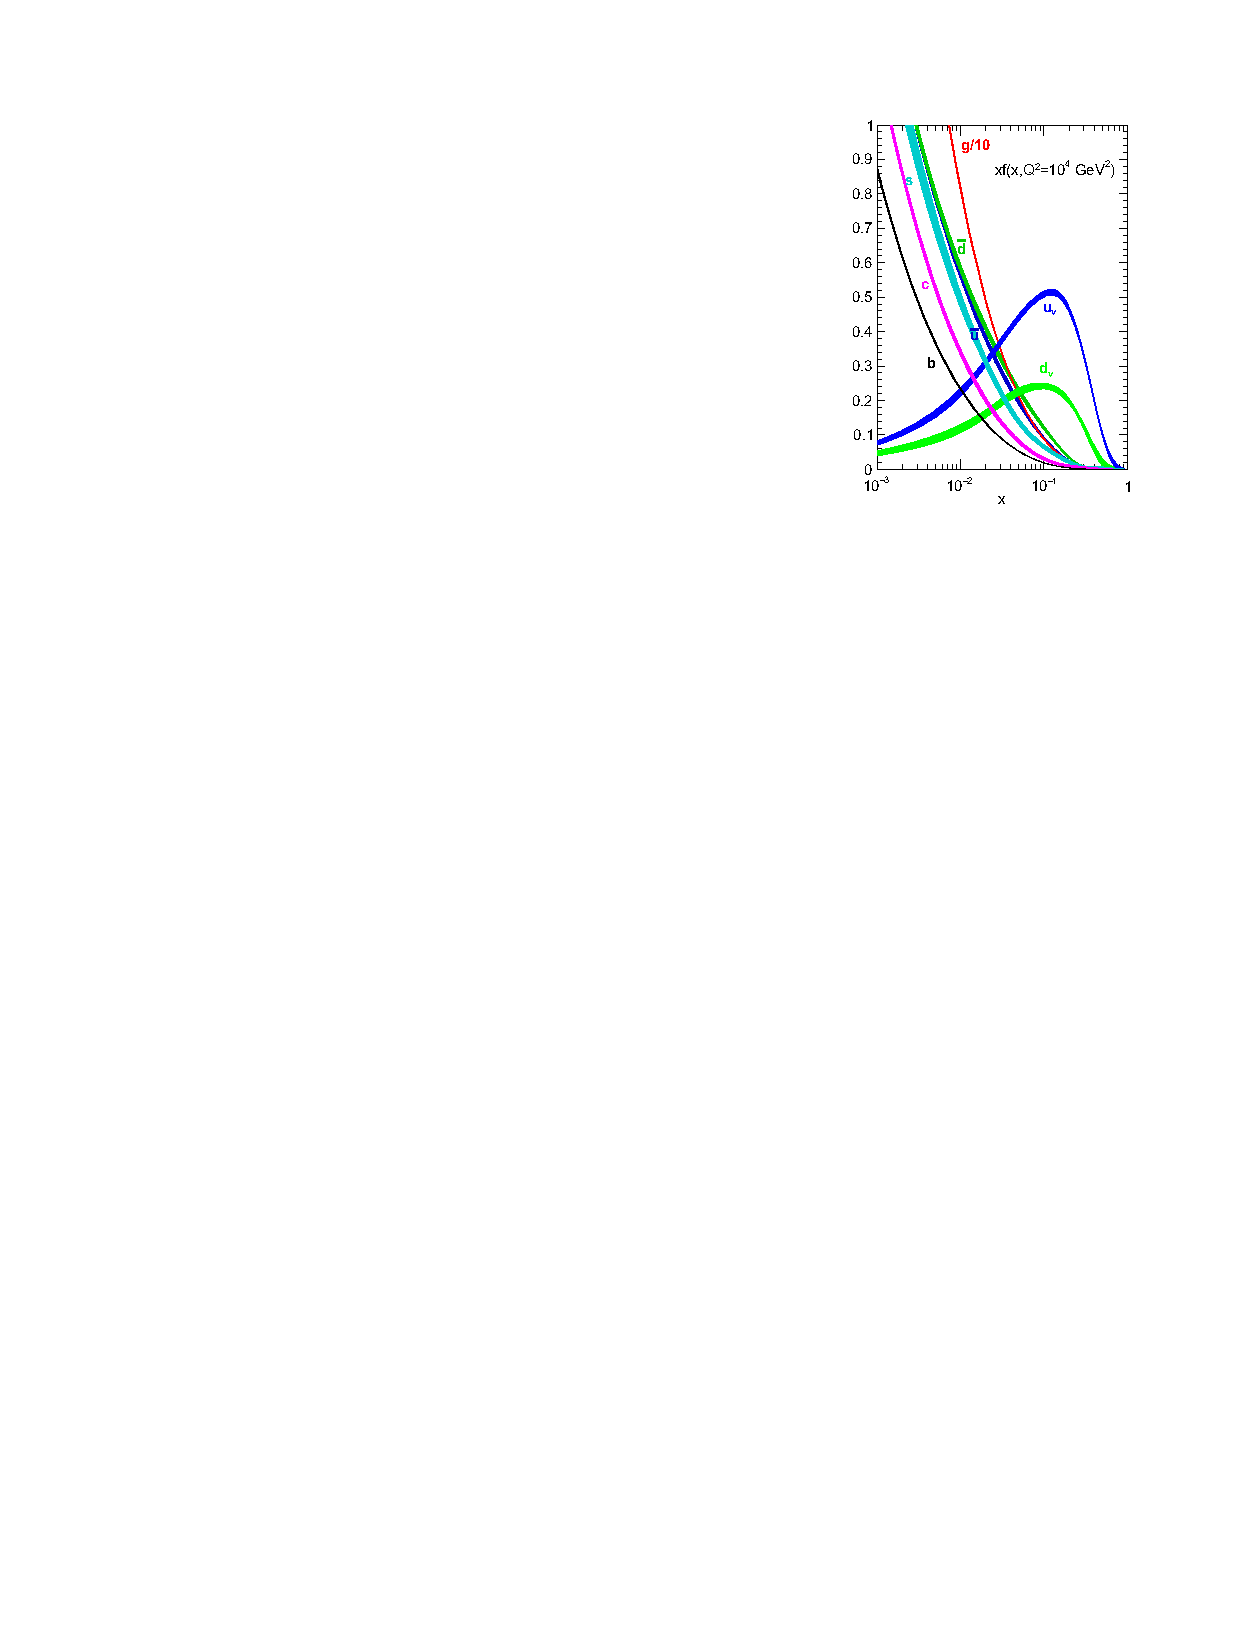
\includegraphics[height=7.8cm]{fig/intro/pdf_NNPDF3.1_NNLO_Q2-10000.pdf}
  %\vspace{0mm}
  \caption{
Plot of the proton PDF $f_p(x,Q^2)$ times the momentum fraction $x$ as calculated by NNPDF3.1 at NNLO accuracy in perturbation theory for $Q^2 = 10\GeV^2$ (left) and $Q^2 = 10^4\GeV^2$ (right).
Adapted from~\cite{NNPDF31}.
  }\label{fig:pdfs}
  %\vspace{-8mm}
\end{figure*}




This follows from the factorization theorem~\cite{PDF_factorization1,PDF_factorization2}, which provides a formula to calculate the cross sections of a hard process with an integral of the form
\begin{equation}
  \sigma(\Pp\Pp\to X + Y)
  = \sum_{i,j} \int_0^1\!\int_0^1 f_i(x_1,Q^2) f_j(x_2,Q^2) \hat\sigma_{ij\to X}(x_1,x_2,Q^2)\dd{x_1}\dd{x_2},
\end{equation}
where $\sigma_{ij\to X}(x_1,x_2,Q^2)$ is the parton-level cross section of the hard process, $i+j \to X$,
and parton $i$ ($j$) carries a fraction $x_1$ ($x_2$) of the momentum of its mother proton.

